\documentclass[12pt]{beamer}
\usetheme{CambridgeUS}
\usepackage[utf8]{inputenc}
\usepackage[spanish]{babel}
\usepackage{amsmath}
\usepackage{amsfonts}
\usepackage{amssymb}
\usepackage{graphicx}
\author{Kevin Garcia - Alejandro Vargas - Alejandro Soto}
\title{Muestreo por importancia}
%\setbeamercovered{transparent} 
%\setbeamertemplate{navigation symbols}{} 
%\logo{} 
%\institute{} 
%\date{} 
%\subject{} 
\begin{document}

\begin{frame}
\titlepage
\end{frame}

%\begin{frame}
%\tableofcontents
%\end{frame}
\begin{frame}
\frametitle{Contenido}
\begin{itemize}
\item Introducción
\item Teoría
\item Algoritmo
\item Ejemplos
\end{itemize}
\end{frame}

\begin{frame}
\frametitle{Introducción}
~\\Aunque hay varios métodos para simular muestras de varias distribuciones, generalmente no es posible obtener una muestra i.i.d. directamente de la distribución a posteriori $h(\theta|x)$ y así hay necesidad de encontrar estrategias alternativas. Por ejemplo, una de esas estrategias posibles es la de simular de una distribución 'semejante' a la distribución a posteriori, para ello surge el muestreo por importancia que se tratará en esta presentación.
\end{frame}

\begin{frame}
\frametitle{Teoría}
~\\Sea $p(\theta)$ una función de densidad de la cual es fácil simular valores y que aproxime $h(\theta|x)=cf(x|\theta)h(\theta)$. Entonces
$$\int g(\theta)h(\theta|x)d\theta=\frac{\int g(\theta)f(x|\theta)h(\theta)d\theta}{\int f(x|\theta)h(\theta)d\theta}$$
$$\int g(\theta)h(\theta|x)d\theta=\frac{\int g(\theta)\frac{f(x|\theta)h(\theta)}{p(\theta)}p(\theta)d\theta}{\int\frac{f(x|\theta)h(\theta)}{p(\theta)}p(\theta)d\theta}$$
$$\int g(\theta)h(\theta|x)d\theta=\frac{\int g(\theta)\omega(\theta)p(\theta)d\theta}{\int \omega(\theta)p(\theta)d\theta}$$
\end{frame}

\begin{frame}
\frametitle{Teoría}
~\\ Si se obtiene una muestra $\theta_{1},\theta_{2},...,\theta_{n}$ de $p(\theta)$, se puede aplicar el método de Monte Carlo, obteniéndose entonces como aproximación de $E[g(\theta)|x]$
$$\hat{E}[g(\theta)|x]=\frac{1}{\sum\limits_{i=1}^{n}\omega_{1}}\sum\limits_{i=1}^{n}\omega_{i}g(\theta_{i})$$
~\\donde $\omega_{i}=f(x|\theta_{i})h(\theta_{i})/p(\theta_{i})$

~\\El método de muestreo por importancia atribuye asi mas peso a regiones donde $p(\theta)<h(\theta|x)$ y menos peso a regiones donde $p(\theta)>h(\theta|x)$. Geweke(1989) muestra que si el soporte de $p(\theta)$ incluye el soporte de $h(\theta|x)$, los $\theta_{i}$ son una muestra i.i.d. de $p(\theta)$, y $\int g(\theta)h(\theta|x)d\theta$ existe y es finita, entonces
\end{frame}

\begin{frame}
\frametitle{Teoría}
$$\frac{1}{\sum\limits_{i=1}^{n}\omega_{i}}\sum\limits_{i=1}^{n}\omega_{i}g(\theta_{i}) \rightarrow \int g(\theta)h(\theta|x)d\theta$$
~\\Con un error estándar de Monte Carlo estimado por:
$$\frac{1}{\sum\limits_{j=1}^{n}\omega_{j}}\left[\sum\limits_{i=1}^{n}\left\lbrace g(\theta_{i})-\frac{1}{\sum\limits_{j=1}^{n}\omega_{j}}\sum\limits_{i=1}^{n}\omega_{i}g(\theta_{i})\right\rbrace^{2}\omega_{i}^2\right]^{1/2} $$
\end{frame}

\begin{frame}
~\\La razón de convergencia depende de cuán bien $p(\theta)$, la función de importancia, imita $h(\theta|x)$. "Buenas" propiedades de la función de importancia son: (i) simplicidad en la generación de números pseudo-aleatorios; (ii) tener colas más pesadas que $h(\cdot|x)$; (iii) ser una buena aproximación a $h(\cdot|x)$
\end{frame}

\begin{frame}
\frametitle{Teoría}
~\\ Se debe señalar que para aplicar esta metodologia sólo hay necesidad de exigir que $h(\theta|x)$ sea conocida a menos de la constante de proporcionalidad, es decir, basta considerar $f(\theta|x)h(\theta)$.Esta observación, también aplicable a la función de importancia, es importante ya que evita la necesidad de calcular la integral necesaria para la obtención de la respectiva constante de proporcionalidad.
\end{frame}

\begin{frame}
\frametitle{Algoritmo}
\begin{itemize}
\item[1.]Simular $\theta_{1},\theta_{2},...,\theta_{m}\sim iid$  $p(\theta)$
\item[2.]Se calcula $\omega_{i}=\frac{h(\theta_{i}|y)}{p(\theta_{i})}$
\item[3.]Se calcula $\frac{1}{\sum_{i=1}^{m}\omega_{i}}\sum_{i=1}^{m}\omega_{i}g(\theta_{i})$, con
\item $g(\theta)=\theta$ para el cálculo aproximado del valor medio de la distribución a posteriori
\item $g(\theta)=\theta^{2}$ para obtener una aproximación de $E(\theta^2)$ de la distribución a posteriori.
~\\Entonces, $V(\theta)=E(\theta^2)-E^2(\theta)$
\end{itemize}
\end{frame}

\begin{frame}
\frametitle{Ejemplo 1}
~\\Sea $X_{i}\sim N(x_{i}|\theta,1)$. La función de verosimilitud es una distribución $N(\bar{x}|\theta,\frac{1}{n})$. Y tomando una distribución a priori $\pi(\theta)\propto 1$. Se quiere estimar $E(\theta|x,\sigma^2)$.\\
~\\Para este ejemplo se utilizo una función de importancia $p(\theta)\sim t_{n}$
~\\Entonces tenemos que $\theta|x,\sigma^2\sim N(\bar{x},\frac{1}{n})$
~\\Para tener el $\bar{x}$ y $\sigma^2$ generamos 10000 valores de x con distribución N(0,1), los resultados fueron:
$$\bar{x}=0.007557463, \sigma^2=\frac{1}{10000}=0.0001$$
\end{frame}

\begin{frame}
\frametitle{Ejemplo 1}
~\\Generamos 10000 $\theta_{i}$ con distribución $p(\theta)\sim t_{n}$
~\\Posteriormente se calculo $\omega_{i}=\frac{f(\theta_{i}|x,\sigma^2)}{p(\theta_{i})}$
~\\Finalmente para estimar la esperanza a posteriori, se calculo $\frac{1}{\sum\limits_{i=1}^{N}\omega_{i}}\sum\limits_{i=1}^{N}\omega_{i}\theta_{i}=0.008330487$
~\\Y, para estimar la varianza a posteriori, se calculo $\frac{1}{\sum\limits_{i=1}^{N}\omega_{i}}\sum\limits_{i=1}^{N}\omega_{i}\theta_{i}^2=0.0001650637$
\end{frame}

\begin{frame}
\frametitle{Ejemplo 1}
Comparando los resultados, tenemos:
\begin{tabular}{|c|c|c|}
\hline 
 & $E(\theta|x,\sigma^2)$ & $V(\theta|x,\sigma^2)$ \\ 
\hline 
Teorica & 0.007557463 & 0.0001 \\ 
Función de importancia $t_{n}$ &  0.008330487 & 0.0001650637 \\ 
\hline 
\end{tabular} 
\end{frame}

\begin{frame}
\frametitle{Ejemplo 2}
~\\ Usando una función de importancia uniforme aproximar la media y la varianza de la distribución a posteriori de $\theta$, para la funcion a posteriori $f(\theta|x)\propto \theta^9(1-\theta)^3, 0<\theta<1$. Para obtener la media y la varianza a posteriori:
~\\Generamos 10000 $\theta_{i}$ con distribución $p(\theta)\sim U(0,1)$
~\\Posteriormente se calculo $\omega_{i}=\frac{f(\theta_{i}|x,\sigma^2)}{p(\theta_{i})}$
~\\Finalmente para estimar la esperanza a posteriori, se calculo $\frac{1}{\sum\limits_{i=1}^{N}\omega_{i}}\sum\limits_{i=1}^{N}\omega_{i}\theta_{i}=0.7324333$
~\\Y, para estimar la varianza a posteriori, se calculo $\frac{1}{\sum\limits_{i=1}^{N}\omega_{i}}\sum\limits_{i=1}^{N}\omega_{i}\theta_{i}^2=0.5489597$
~\\Entonces, $V(\theta|x,\sigma^2)=0.01250114$
\end{frame}

\begin{frame}
\frametitle{Ejemplo 2}
Comparando los resultados, tenemos:
\begin{tabular}{|c|c|c|}
\hline 
 & $E(\theta|x,\sigma^2)$ & $V(\theta|x,\sigma^2)$ \\ 
\hline 
Teorica & 0.7142857 & 0.01360544 \\ 
Función de importancia Uniforme &  0.7324333 & 0.01250114 \\ 
\hline 
\end{tabular} 
\end{frame}

\begin{frame}
\frametitle{Ejemplo 3}
~\\Veamos como hacer uso del concepto de función de importancia para obtener la distribución a posteriori y calcular el valor medio y varianza a posteriori. Supongamos que se tiene una función de densidad a posteriori de la siguiente forma:
$$h(\theta|y)\propto(2+\theta)^{y_{1}}(1-\theta)^{y_{2}+y_{3}+b-1}\theta^{y_{4}+a-1},   0\leq\theta\leq1 $$
~\\y
$$L(\theta|y)=log h(\theta|y)\propto y_{1}log(2+\theta)+(y_{2}+y_{3}+b-1)log(1-\theta)+(y_{4}+a-1)log(\theta)$$
$$L'(\theta)=\frac{y_{1}}{2+\theta}-\frac{y_{2}+y_{3}+b-1}{1-\theta}+\frac{y_{4}+a-1}{\theta}$$
$$L''(\theta)=\frac{y_{1}}{(2+\theta)^2}-\frac{y_{2}+y_{3}+b-1}{(1-\theta)^2}+\frac{y_{4}+a-1}{\theta^2}$$
\end{frame}

\begin{frame}
~\\Una función de importancia bastante utilizada es la función de densidad Normal, ya que lo que se pretende es simular de una distribución que aproxime la distribución a posteriori. Sin embargo hay situaciones en que la aproximación por la normal no es adecuada y por lo tanto otra función de importancia debe ser considerada. Una representación gráfica de la verosimilitud puede ayudar en la selección; en este caso, dado que el parámetro para el que se pretende obtener la distribución a posteriori varia en el intervalo $[0,1]$, la función de densidad Beta también puede considerarse adecada como candidata a función de importancia.
~\\Se procederá entonces al método de muestreo por importancia utilizando las dos funciones, Normal y Beta, para las dos muestras en estudio. Para ello es necesario simular muestras de esas distribuciones. Se designa por $p(\theta)$ la función de importancia en consideración. 
\end{frame}

\begin{frame}
~\\Como se dijo anteriormente, sea $\hat{\theta}$ el valor de $\theta$ para el cual $L'(\theta)=0$, y $\hat{\sigma^2}=\left\lbrace -L''(\hat{\theta})\right\rbrace^{-1}$. Se consideran estos valores como aproximaciones, respectivamente, para el valor medio y la varianza de la distribución a posteriori. Estos valores serán necesarios para obtener los parámetros de las distribuciones a simular. Se procede entonces de la siguiente manera:
\begin{itemize}
\item[1.]Se simula $\theta_{1},\theta_{2},...,\theta_{m}\sim iid$  $p(\theta)$
\item[2.]Se calcula $\omega_{i}=\frac{h(\theta_{i}|y)}{p(\theta_{i})}$
\item[3.]Se calcula $\frac{1}{\sum_{i=1}^{m}}\sum_{i=1}^{m}\omega_{i}g(\theta_{i})$, con
\item $g(\theta)=\theta$ para el cálculo aproximado del valor medio de la distribución a posteriori
\item $g(\theta)=\theta^{2}$ para obtener una aproximación de la varianza de la distribución a posteriori.
\end{itemize}
\end{frame}

\begin{frame}
\frametitle{Ejemplo 3}
\begin{figure}[!h]
    \begin{center}
        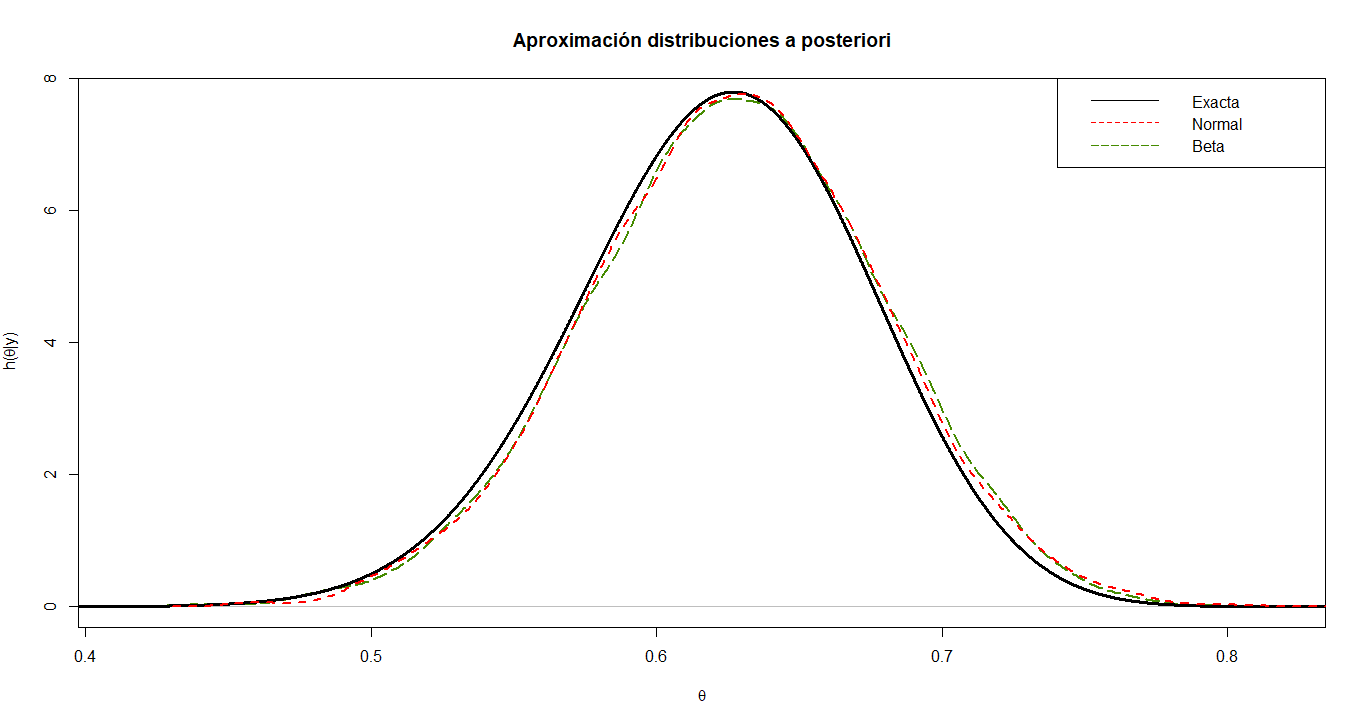
\includegraphics[width=12.5cm]{imagenes/ej3.png}
        \caption{Comportamiento de la distribución Poisson variando $\lambda$}
        \label{fig:Densidad}
    \end{center}
\end{figure}
\end{frame}

\begin{frame}
\frametitle{Ejemplo 3}
\center
\begin{tabular}{|p{2.2cm}|cc|cc|}
\hline 
 & N=197 &  & N=20 &  \\ 
\hline 
Función de importancia & $E(\theta|y)$ & $V(\theta|y)$ & $E(\theta|y)$ & $V(\theta|y)$ \\ 
\hline 
Beta &  0.6230844 & 0.002572936 & 0.8460755 & 0.01190065 \\ 
\hline 
Normal & 0.6232495 & 0.00257044 & 0.8862506 & 0.00043632 \\ 
\hline 
Exacta & 0.6228062 & 0.002594837 & 0.8311239 & 0.01165126 \\ 
\hline 
\end{tabular} 
\end{frame}


\begin{frame}
~\\Como se puede observar, en el caso de la primera muestra, el método de muestreo por importancia proporciona buenas aproximaciones, para ambas funciones de importancia consideradas.  El mismo ya no ocurre en el caso de la segunda muestra, donde la función Normal (incluso truncada) no es adecuada. Sin embargo, la función Beta proporciona una buena aproximación. 
\end{frame}

\begin{frame}[fragile]
\frametitle{Códigos R}
\framesubtitle{Ejemplo 1}
\begin{verbatim}
#Ejemplo 1:
N=10000
X<-rnorm(N)
xbarra=mean(X)
varianza=1/N
thetai<-rt(N,N)
w<-dnorm(thetai,xbarra,sqrt(varianza))/dt(thetai,N)
E<-(1/sum(w))*(sum(w*thetai))
V<-(1/sum(w))*(sum(w*(thetai^2)))
\end{verbatim}
\end{frame}

\begin{frame}[fragile]
\frametitle{Códigos R}
\framesubtitle{Ejemplo 2}
\begin{verbatim}
#Ejemplo 2:
funcion<-function(x){(x^9)*((1-x)^3)}
tetai<-runif(N)
w1<-funcion(tetai)/dunif(tetai)
E1<-(1/sum(w1))*(sum(w1*tetai))  #Esperanza estimada
V1<-(1/sum(w1))*(sum(w1*(tetai^2))) #Varianza estimada
\end{verbatim}
\end{frame}
\end{document}